\documentclass[tikz, border=5pt]{standalone}

\begin{document}
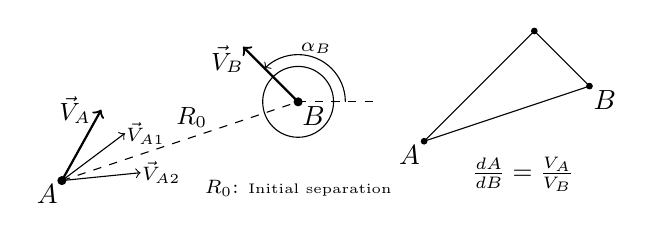
\begin{tikzpicture}

    %% Collision cone

    \begin{scope}
        % Mass A
        \coordinate (A) at (0,0);
        \draw[fill] (A) circle (0.05) node[below left=-2] {\( A \)};

        % Mass B
        \coordinate (B) at (3,1);
        \draw[fill] (B) circle (0.05) node[below right=-2] {\( B \)};

        \draw (B) circle (0.45);
        \draw[dashed] (B) -- ++(1,0);

        % Line of separation
        \draw[dashed] (A) -- (B) node[pos=0.55, above] {\small \( R_0 \)};

        % Angles
        \draw[->] (B) ++(0.6,0) arc (0:135:0.6) node[midway, above=-2] {\scriptsize \( \alpha_B \)};

        % Vectors
        \draw[->, thick] (A) -- ++(0.5,0.9) node[left] {\small \( \vec{V}_A \)};
        \draw[->, thick] (B) -- ++(-0.7,0.7) node[below left=-4] {\small \( \vec{V}_B \)};
        \draw[->] (A) -- ++(0.8,0.6) node[right=-3] {\scriptsize \( \vec{V}_{A 1} \)};
        \draw[->] (A) -- ++(1,0.1) node[right=-3] {\scriptsize \( \vec{V}_{A 2} \)};

        % Legend
        \node at (3,-0.1) {\scriptsize \( R_0 \): \tiny Initial separation};
    \end{scope}

    \begin{scope}[xshift=4.6cm, yshift=0.5cm, scale=0.7]
        \coordinate (A) at (0,0);
        \coordinate (B) at (3,1);
        \coordinate (C) at (2,2);

        \draw[fill] (A) circle (0.05) node[below left=-2] {\( A \)};
        \draw[fill] (B) circle (0.05) node[below right=-2] {\( B \)};
        \draw[fill] (C) circle (0.05);

        \draw (A) -- (B) -- (C) -- cycle;

        \node at (1.8,-0.6) {\small \( \frac{dA}{dB} = \frac{V_A}{V_B} \)};
    \end{scope}

\end{tikzpicture}
\end{document}
